\documentclass{refrep}
\settextfraction{.9}
\usepackage[dvipsnames]{xcolor}
\usepackage{extramarks}
\usepackage{amsmath}
\usepackage{amsthm}
\usepackage{amsfonts}
\usepackage{tikz}
\usepackage[plain]{algorithm}
\usepackage{algpseudocode}
\usepackage{listings}
\usepackage{datetime}
\usepackage{float}
\usepackage{graphicx}
\usepackage[export]{adjustbox}
\usepackage[tableposition=below]{caption}
\usepackage{contour}
\usepackage{longtable,tabu}
\makeatletter
\newcount\dirtree@lvl
\newcount\dirtree@plvl
\newcount\dirtree@clvl
\def\dirtree@growth{
  \ifnum\tikznumberofcurrentchild=1\relax
  \global\advance\dirtree@plvl by 1
  \expandafter\xdef\csname dirtree@p@\the\dirtree@plvl\endcsname{\the\dirtree@lvl}
  \fi
  \global\advance\dirtree@lvl by 1\relax
  \dirtree@clvl=\dirtree@lvl
  \advance\dirtree@clvl by -\csname dirtree@p@\the\dirtree@plvl\endcsname
  \pgf@xa=.25cm\relax
  \pgf@ya=-.5cm\relax
  \pgf@ya=\dirtree@clvl\pgf@ya
  \pgftransformshift{\pgfqpoint{\the\pgf@xa}{\the\pgf@ya}}%
  \ifnum\tikznumberofcurrentchild=\tikznumberofchildren
  \global\advance\dirtree@plvl by -1
  \fi
}

\tikzset{
  dirtree/.style={
    growth function=\dirtree@growth,
    every node/.style={anchor=north},
    every child node/.style={anchor=west},
    edge from parent path={(\tikzparentnode\tikzparentanchor) |- (\tikzchildnode\tikzchildanchor)}
  }
}

\makeatother
\graphicspath{ {images/vc707/} {images/vc709/} {images/qsys/} {images/ipc/} {images/perf/} {images/}}
\newcommand{\TinkerVersion}{Tinker 1.0 (Beta)}
\newcommand{\figurewidth}{350px}
\newcommand{\Directory}[1]{\textit{#1}}
\newcommand{\EnvVariable}[1]{\textbf{#1}}
\newcommand{\TermCmd}[1]{\$ \texttt{#1}}
\newcommand{\TODO}[1]{\textbf{\color{red}{#1}}}
\newcommand{\Keyword}[1]{\textbf{\color{BlueViolet}{#1}}}
\newcommand{\Subst}[1]{\textbf{\textless{#1}\textgreater}}
\newcommand{\ConfigSetting}[1]{\textbf{#1}}

\title{{\TinkerVersion} Documentation}
\author{Dustin Richmond}
\date{\today}
\graphicspath{{./figures/}}
\begin{document}

\maketitle
\pagebreak
\tableofcontents

\chapter{License}
\label{Chapter:License}

Copyright (c) 2016, The Regents of the University of California All rights
reserved.

Redistribution and use in source and binary forms, with or without modification,
are permitted provided that the following conditions are met:

\begin{itemize}
    \item Redistributions of source code must retain the above copyright
      notice, this list of conditions and the following disclaimer.

    \item Redistributions in binary form must reproduce the above
      copyright notice, this list of conditions and the following
      disclaimer in the documentation and/or other materials provided
      with the distribution.

    \item Neither the name of The Regents of the University of California
      nor the names of its contributors may be used to endorse or
      promote products derived from this software without specific
      prior written permission.
\end{itemize}

THIS SOFTWARE IS PROVIDED BY THE COPYRIGHT HOLDERS AND CONTRIBUTORS ``AS IS''
AND ANY EXPRESS OR IMPLIED WARRANTIES, INCLUDING, BUT NOT LIMITED TO, THE
IMPLIED WARRANTIES OF MERCHANTABILITY AND FITNESS FOR A PARTICULAR PURPOSE ARE
DISCLAIMED. IN NO EVENT SHALL REGENTS OF THE UNIVERSITY OF CALIFORNIA BE LIABLE
FOR ANY DIRECT, INDIRECT, INCIDENTAL, SPECIAL, EXEMPLARY, OR CONSEQUENTIAL
DAMAGES (INCLUDING, BUT NOT LIMITED TO, PROCUREMENT OF SUBSTITUTE GOODS OR
SERVICES; LOSS OF USE, DATA, OR PROFITS; OR BUSINESS INTERRUPTION) HOWEVER
CAUSED AND ON ANY THEORY OF LIABILITY, WHETHER IN CONTRACT, STRICT LIABILITY, OR
TORT (INCLUDING NEGLIGENCE OR OTHERWISE) ARISING IN ANY WAY OUT OF THE USE OF
THIS SOFTWARE, EVEN IF ADVISED OF THE POSSIBILITY OF SUCH DAMAGE.
\pagebreak

\chapter{Setup and Installation}
\label{Chapter:Setup}
\section{Conventions}
\label{Chapter:Setup:Section:Conventions}
In this user guide, we use the following conventions:
\begin{center}
  \begin{tabular}{ | l | l |}
    \hline
    Object & Example \\ \hline
    Directories and Paths & \Directory{tinker/boards/14.1}  \\ \hline
    Configuration Setting & \ConfigSetting{Number of Lanes} \\ \hline
    Terminal Command, Code Snippet & \TermCmd{echo ``Hello World''}\\ \hline
    Substituted Text & \Subst{System ID} \\ \hline
  \end{tabular}
\end{center}

\section{Dependencies}
\label{Chapter:Setup:Section:Dependencies}

The Tinker project has three dependencies. These should be installed by the user
prior to generating a board using an appropriate package manager or installation
executable.

\begin{itemize}
\item TclXML >= 3.2 (typically tclxml)
\item Quartus
\item
\end{itemize}

\section{Installation}
\label{Chapter:Setup:Section:Installation}

To install tinker, simply clone the git repository:\\

\TermCmd{git clone https://github.com/drichmond/tinker.git}\\

\section{Environment}
\label{Chapter:Setup:Section:Environment}
Tinker relies on two environment variables. In a bash environment set these to
appropriate values using \TermCmd{export} in your bash settings file. The tinker
script will not run unless these variables are set.

\renewcommand{\arraystretch}{1.5}
\begin{longtable}{|p{3cm}|p{10cm}|}
  \hline

  \EnvVariable{TINKER\_PATH} & Path to the local root of the Tinker GitHub
  repository. \\ \hline

  \EnvVariable{TCLXML\_PATH} & Path to the TCL XML Library, a directory containing a
  set of shared objects used by a TCL Shell. This path can be determined in bash
  by running: \TermCmd{locate libTclxml}\\
  

  \hline
  \caption{Environment variables required by the tinker board generator.}
\end{longtable}


\pagebreak
\chapter{Introduction: Tinker}
\label{Chapter:Intro}
\section{Repository Structure}
\label{Chapter:Intro:Section:Structure}
Fig~\ref{Fig:Tinker:DirStructure} shows the directory hierarchy of Tinker. This
instruction manual uses this directory tree when specifying all directory paths.

\begin{itemize}
\item \Directory{boards/} contains all of boards supported by tinker, grouped by Quartus Version
\item \Directory{docs/} contains all of the documentation for this project
\item \Directory{example/} contains a set of example user specifications (written in JSON)
\item \Directory{python/} contains all of the Python files necessary for running tinker
\item \Directory{tcl/} contains all of the tcl scripts used by Quartus/Qsys during OpenCL Compilation
\item \Directory{tests/} contains a set of tests that can be used to test a custom board. 
\end{itemize}

\begin{figure}[H]
  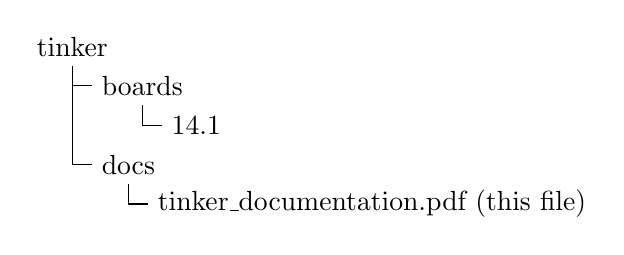
\begin{tikzpicture}[dirtree]
    \node {tinker}
    child { 
      node {boards}
      child { 
        node {14.1} 
      }
    }
    child { 
      node {docs}
      child { 
        node {tinker\_documentation.pdf (this file)}
      }
    };
  \end{tikzpicture}
  \caption{Directory hierarchy of the RIFFA \TinkerVersion~distribution} \label{Fig:Tinker:DirStructure}
\end{figure}

\section{Release Notes}
\subsection{Tinker 1.0 (Beta)}
\begin{itemize}
  \item Beta Release: There may be bugs in this version. 
  \item Support for Terasic DE5Net Board in Quartus 14.1
\end{itemize}

\pagebreak
\chapter{Generating and Compiling and Installing a Custom Board}
\label{Chapter:Generating}
% Tinker is a shell-based utility that reads high-level specifications and
% generates custom boards.

The tinker utility has three options which are detailed using the -h flag, shown
in Listing~\ref{Listing:Tinker:Help}. An incorreclty configured environment will
produce an error. If this happens, return to Section~\ref{Chapter:Setup:Section:Environment}.

\begin{lstlisting}[language=bash,basicstyle=\footnotesize\ttfamily,commentstyle=\color{red},
    label=Listing:Tinker:Help,captionpos=b,
    caption=Output from running ./tinker -h in a correctly configured environment,frame=single]
  $ ./tinker -h
  usage: tinker [-h] [-l] [-i <version> <board_name>]
              [-g <path-to-specification> <version> <board_name>]

  Generate a Board Support Package for Altera's OpenCL Compiler

  optional arguments:
    -h, --help            show this help message and exit
    -l, --list-boards     List the available board skeletons available to Tinker
    -i <version> <board_name>
                          Get info about a specific board and version
    -g <path-to-specification> <version> <board_name>
                          Generate a Board Support Package (BSP) using the
                          specification within the text file
\end{lstlisting}



A Board Support Package contains three parts:
\begin{enumerate}
\item Libraries and drivers for communication 
\item A hardware system, project file, top level file, with kernel
  interfaces.
\item A metadata with hardware interfaces, address map, and data
  layout for the OpenCL Compiler.
\end{enumerate}

Tinker generates a memory architectures which affect items 2 and 3 above. 
A memory architecture defines how available memory interfaces
are grouped into memory systems. Figure~\ref{Fig:Tinker:OpenCLBSP} shows a
memory architecture with two memory systems.

\begin{figure}[h]
\centering
\includegraphics[width=3in]{OpenCLBSP.pdf}
\caption{Hardware components of an OpenCL Board Support Package. Green wires
  indicate data busses, blue indicates clock networks.}
\label{Fig:Tinker:OpenCLBSP}
\end{figure}

Figure~\ref{Fig:Tinker:OpenCLBSP} shows a simple memory architecture with two
memory systems, with two memory interfaces in each system. A memory system is a
grouping of memory interfaces of identical type that provide a single unified
address space to the user kernel. A memory system defines the interleaving
pattern, bandwidth, and data placement.  Data is interleaved across banks within
a memory system to improve random access performance, but is not visible to the
user. For more information about the effects of interleaving please read about
interleaved bytes in the Altera SDK for OpenCL Custom Platform Toolkit User
Guide\footnote{https://www.altera.com/content/dam/altera-www/global/en\_US/pdfs/literature/hb/opencl-sdk/ug\_aocl\_custom\_platform\_toolkit.pdf}.



\section{Specifying a Custom Board}
\label{Chapter:Generating:Sec:Generation}
To generate a custom board, a user writes a high level specficiation using the
key-value pairs defined in this section. These are organized in Javascript
Object Notation (JSON), as shown in the example in
Listing~\ref{Listing:Tinker:Specification}. Example specifications can be found
in the \Directory{example} directory.

Executing \TermCmd{tinker -i} is useful for obtaining about the memory
interfaces available on a supported board. Obtaining information about the
de5net board for Quartus Version 14.1 gives the output shown in
Listing~\ref{Listing:Tinker:Info}.

\begin{lstlisting}[language=bash,basicstyle=\footnotesize\ttfamily,commentstyle=\color{red},
    label=Listing:Tinker:Info,captionpos=b,
    caption=Output from running ./tinker -i 14.1 de5net in a correctly configured environment,frame=single]
  $ ./tinker -i 14.1 de5net
    Getting Info for Board de5net, Version 14.1
    Available Memories: ['DDR3', 'QDRII']
    Showing info for memory type QDRII:
            Number of Interfaces: 4
            Interface ID: a
                    Size: 0x800000 (8388608 bytes)
                    Max Freq: 450 MHz
                    Associated Interfaces: ['b', 'c']
                    Roles: ['primary', 'secondary', 'independent']
                    Ports: ['r', 'w']
                    Bandwidth: 108000 Bytes/Sec
            Interface ID: c
                    Size: 0x800000 (8388608 bytes)
                    Max Freq: 450 MHz
                    Associated Interfaces: ['a', 'b']
                    Roles: ['primary', 'secondary', 'independent']
                    Ports: ['r', 'w']
                    Bandwidth: 108000 Bytes/Sec
            Interface ID: b
                    Size: 0x800000 (8388608 bytes)
                    Max Freq: 450 MHz
                    Associated Interfaces: ['a', 'c']
                    Roles: ['primary', 'secondary', 'independent']
                    Ports: ['r', 'w']
                    Bandwidth: 108000 Bytes/Sec
            Interface ID: d
                    Size: 0x800000 (8388608 bytes)
                    Max Freq: 450 MHz
                    Associated Interfaces: []
                    Roles: ['primary']
                    Ports: ['r', 'w']
                    Bandwidth: 108000 Bytes/Sec
    Showing info for memory type DDR3:
            Number of Interfaces: 2
                    Interface ID: a
                    Size: 0x80000000 (2147483648 bytes)
                    Max Freq: 800 MHz
                    Associated Interfaces: ['b']
                    Roles: ['primary', 'secondary', 'independent']
                    Ports: ['rw']
            Bandwidth: 12800000000 Bytes/Sec
                    Interface ID: b
                    Size: 0x80000000 (2147483648 bytes)
                    Max Freq: 800 MHz
                    Associated Interfaces: ['a']
                    Roles: ['primary', 'secondary', 'independent']
                    Ports: ['rw']
                    Bandwidth: 12800000000 Bytes/Sec
  
\end{lstlisting}

Listing~\ref{Listing:Tinker:Info} demonstrates that the DE5Net board provides
six memories: two DDR Memories, and four QDR Memories. The two DDR Memories: 'a'
and 'b'. Each DDR memory has 2 gigibytes of storage (Size: 0x80000000
(2147483648 bytes)), one bidirectional port (Ports: ['rw']), and a maximum
frequency of 800 MHz. The DE5Net also has 4 QDR Memories: 'a', 'b', 'c', and
'd'. Each QDR Memory has 8 mebibytes of storage (Size: 0x800000 (8388608
bytes)), one read port and one write port (Ports: ['r', 'w']), and a maximum
frequency of 450 MHz.

A user can use the information shown in Listing~\ref{Listing:Tinker:Info} to
create a specification as shown in Listing~\ref{Listing:Tinker:Specification}.

% TODO: Potential Widths need to be printed with the info (somehow)

\lstinputlisting[language=Java,basicstyle=\footnotesize\ttfamily,commentstyle=\color{red},
    label=Listing:Tinker:Specification,captionpos=b,
    caption=Example board specification provided by the user with two 2-Gigibyte DDR3 interfaces,frame=single, stringstyle=\color{OliveGreen}]
{../example/2XD2GB.json}

The board properties are defined in the first level of a specification. The keys
and associated values in Table~\ref{Table:Tinker:Board} are used to define board
properties. See Listing~\ref{Listing:Tinker:Specification} for examples of each
key.

\renewcommand{\arraystretch}{1.5}
\begin{longtable}{|p{3cm}|p{10cm}|}
  \hline

  \Keyword{Name} & A string defining the name of the specification. When
  generating a board, the board name will be prepended to this name to create
  the final name. 
  \\ \hline

  \Keyword{Systems} & A numeric list of all memories on the board identified by
  their \Subst{System ID} (See below)\\

  \hline

  \Keyword{\Subst{System ID}} & E.g. 0, 1, 2, 3. All memory systems enumerated
  in the \Keyword{Systems} list above must be enumerated the board level of the
  specification.\\

  \hline
  \caption{Key-value pairs that define a Board in the board specification JSON
    file shown in Listing~\ref{Listing:Tinker:Specification}}
  \label{Table:Tinker:Board}
\end{longtable}

\begin{figure}[h]
\centering
\includegraphics[width=3in]{OpenCLMemorySystem.pdf}
\caption{A simple memory system instantiating $M$ memory interfaces, each
  providing a kernel interface, and a bank divider providing a contiguous memory
  space on top of an interleaving pattern}
\label{Fig:Tinker:MemSys}
\end{figure}

Each \Keyword{\Subst{System ID}} contains a second level of parameters that
define a memory system. Figure~\ref{Fig:Tinker:MemSys} shows a memory system
composed of $M$ memory interfaces and A memory interface is a physical package,
e.g. a DIMM. A memory system defines how low-level resources like PLL's, DLL's
are shared to reduce resource usage and clock crossings. Each of the memory
interfaces in a memory system provide a single non-uniform access memory port to
compiler generated logic.

Each memory system has a role: Primary or Secondary. A primary memory system
provides a clock output to drive the DMA engine. The clock frequency of a memory
system is determined by the maximum frequency multiplied by the fabric ratio
(Quarter, Half, Full). It is advantageous to have the DMA engine run at least as
fast as the PCIe Endpoint (typically 250 MHz). \TODO{Change to Quarter, half, full}

The properties of each memory system are defined in the second level of a
specification. The keys and associated values in Table~\ref{Table:Tinker:System}
are used to define memory system properties. See
Listing~\ref{Listing:Tinker:Specification} for examples of each key.

\renewcommand{\arraystretch}{1.5}
\begin{longtable}{|p{3cm}|p{10cm}|}
  \hline

  \Keyword{System} & The numeric ID of the system associated with this level of
  the specification. Must match the \Keyword{\Subst{System ID}} for this level. \\ \hline

  \Keyword{Role} & The role of the memory system. One memory system must be
  primary, and all others must be secondary.\\ \hline

  \Keyword{Primary} & The ID of the primary memory interface in the memory
  system. See Listing~\ref{Listing:Tinker:Info} and
  Table~\ref{Table:Tinker:Interface} for more information\\ \hline

  \Keyword{Type} & The type of the memory system \TinkerVersion supports QDR and
  DDR memory types \\ \hline

  \Keyword{Interfaces} & A list of Memory Interface IDs in this memory
  system. Each memory interface must be associated with all other memory
  interfaces in the system 
  Listing~\ref{Listing:Tinker:Info})\\ \hline

  \Keyword{Width} & The width of the Memory Interface \\ \hline
  
  \Keyword{\Subst{Interface ID}} & Alphabetical ID for memory interfaces
  enumerated in the \Keyword{Interfaces}. All memory interfaces listed in
  \Keyword{Interfaces} above must be enumerated at the memory system level of
  the specification. \\ \hline
  
  \caption{Key-value pairs that define a Memory System in the second level of a
    board specification JSON file shown in
    Listing~\ref{Listing:Tinker:Specification}}
  \label{Table:Tinker:System}
\end{longtable}

A memory interface is a physical package, e.g. a
DIMM. Figure~\ref{Fig:Tinker:MemSys} shows a memory system composed of $M$
memory interfaces.

\begin{itemize}
 \item A \textit{primary} memory instantiates it's own PLL, drives the bank
   divider, and the clock output. It is the master for PLL, DLL, and OCT sharing
   relationships.
 \item A \textit{secondary} memory interface shares all PLLs, DLLs and OCT pins
   from a primary memory interface, and thus operates in the same clock domain.
\item An \textit{independent} memory interface instantiates its own PLL and DLL,
  and can share an OCT pin. An independent memory operates in a separate clock
  domain with clock crossing interfaces.
\end{itemize}

The properties of each memory interface are defined in the third level of a
specification. The keys and associated values in Table~\ref{Table:Tinker:Interface}
are used to define memory interface properties. See
Listing~\ref{Listing:Tinker:Specification} for examples of each key.

\renewcommand{\arraystretch}{1.5}
\begin{longtable}{|p{3cm}|p{10cm}|}

  \hline \Keyword{\Subst{ID}} & The alphabetical ID of the memory
  interface. Must match the \Keyword{\Subst{Interface ID}} key for this
  level. \\ \hline
    
  \Keyword{Role} & The role of the memory interface. Each memory interface must
  be primary, secondary, or independent according to the options showin in
  Listing~\ref{Listing:Tinker:Info}. \\ \hline

  \Keyword{Size} & \TODO{Remove size?} \\  \hline

  \caption{Key-value pairs that define a Memory Interface in the third level of
    a board specification JSON file shown in
    Listing~\ref{Listing:Tinker:Specification}}
  \label{Table:Tinker:Interface}
\end{longtable}

Finally, when a full specification has been designed the user can generate the board. To generate the board, run the \TermCmd{tinker -g} command as follows in Listing~\ref{Listing:Tinker:Generate}

\begin{lstlisting}[language=bash,basicstyle=\footnotesize\ttfamily,commentstyle=\color{red},
    label=Listing:Tinker:Generate,captionpos=b,
    caption=Output from running ./tinker -g examples/2XD2GB.json 14.1 de5net,frame=single]
  $ ./tinker -i 14.1 de5net
    Board de5net_2XD2GB generated
\end{lstlisting}

\section{Installing a Custom Board}
\label{Chapter:Generating:Sec:Installation}

Once a board has been generated, installing the board is a relatively
straightforward process. Assuming that the Terasic DE5Net Board has been
correctly installed, the user has two options: Symlink or Copying. This
instruction manual recommends symlinking.

To install your generated board using the ln command issue the following command
in your terminal from the directory containing the generated board:

\begin{lstlisting}[language=bash,basicstyle=\footnotesize\ttfamily,commentstyle=\color{red},
    label=Listing:Tinker:Install,captionpos=b,
    caption=Installing a board using the ln command in a correctly installed Altera OpenCL Environment,frame=single]
$ ln -s \Keyword{Board Name} $AOCL_BOARD_PACKAGE_ROOT/hardware/\Keyword{Board Name}
\end{lstlisting}

If a symlink is used to install the board the board only needs to be installed
once. Any further modifications and re-generations will automatically propogate
to the Altera OpenCL Compiler.

Alternatively, you can use the cp command to install your board. The downside of
this approach is that everytime a board is regenerated it must be replaced by
re-running the cp command.

\begin{lstlisting}[language=bash,basicstyle=\footnotesize\ttfamily,commentstyle=\color{red},
    label=Listing:Tinker:List,captionpos=b,
    caption=Installing a board using the cp command,frame=single]
  
$ cp -r \Keyword{Board Name} $AOCL_BOARD_PACKAGE_ROOT/hardware/
\end{lstlisting}




To check if your board has been properly installed, run the \TermCmd{aoc
  --list-boards} command shown in Listing~\ref{Listing:Tinker:List}. Your board
should be printed in the command output.

\begin{lstlisting}[language=bash,basicstyle=\footnotesize\ttfamily,commentstyle=\color{red},
    label=Listing:Tinker:List,captionpos=b,
    caption=Output from running aoc --list-boards after correctly installing the de5net\_2XD2GB board from Section~\ref{Chapter:Generating:Sec:Generation},frame=single]
  
  $ aoc --list-boards
  Board list:
  de5net\_2XD2GB

  de5net\_a7
\end{lstlisting}

You can now use your board like any other board provided by the vendor.


%\section{Compiling a Custom Board}
%\label{Chapter:Generating:Sec:Compilation}


\pagebreak
\chapter{Adding Support a New Board}
\label{Chapter:Adding}
\section{Top Level Design File}
\label{Chapter:Adding:Section:Top}
\section{Board XML File}
\label{Chapter:Adding:Section:XML}

\section{Project File}
\label{Chapter:Adding:Section:Project}
\section{Timing Files}
\label{Chapter:Adding:Section:Timing}
\subsection{Memory Interfaces}
\label{Chapter:Adding:Section:Project:Sub:Memories}
\section{Qsys Files}
\label{Chapter:Adding:Section:Qsys}
% Kernel Interface
\section{Installation}
\label{Chapter:Adding:Section:Installation}
\section{Testing}
\label{Chapter:Adding:Section:Testing}
\pagebreak
\chapter{Developer Documentation}
\label{Chap:Tinker:Adding}
\end{document}
